\chapter{Stand der Wissenschaft und Auswahl von Verfahren}

In diesem Kapitel soll der aktuelle Stand der Wissenscahft bezogen auf die in dieser Arbeit verwendeten Klassen von Verfahren betrachtet werden sowie ausgehend von den Anforderungen an das zu entwickelnde System ein passendes Verfahren ausgewählt und im Detail beschrieben werden. An geeigneten Stellen wird auf die im letztten Kapitel dargelegten Grundlagen zurückgegriffen.

\label{cha_state}

\section{SIEM-Systeme}

\label{sec_state_siem}

Zur Zeit gibt es eine vielfältige Auswahl an SIEM-Systemen auf dem Markt, die die grundsätzlichen Aufgaben eines SIEM-Systems erfüllen und über diese hinausgehen: Splunk\footnote{
  https://www.splunk.com
}, QRadar von IBM\footnote{
  https://www.ibm.com/us-en/marketplace/ibm-qradar-siem
} oder ArcSight von Micro Focus\footnote{
  https://software.microfocus.com/en-us/software/siem-security-information-event-management
} sind nur einige Beispiele aus diesem Bereich. \todo{Die Funktionen dieser Systeme sind alle ähnlich/total unterschiedlich/ gehen von bis usw.}

\todo{Umschreiben - OSSIM weil ...}

Die Auswahl an Open-Source-Software in diesem Bereich ist jedoch sehr gering. Eine der wenigen Ausnahmen stellt OSSIM - ein SIEM-System der Firma AlienVault\footnote{
	AlienVault OSSIM: The World’s Most Widely Used Open Source SIEM\\https://www.alienvault.com/products/ossim
} - dar, das auf Basis weiterer quelloffener Lösungen aus dem Netzwerksicherheits-Bereich unter anderem die in Abschnitt \ref{sec_basics_siem} beschriebenen Funktionen bereitstellt. AlienVault bietet zusätzliche eine kommerzielle Variante seines Produkts namens USM an, das insbesondere in den Bereichen Event-Korrelation und Compliance-Reporting die Funktionalität von OSSIM übersteigt. Von der Entwicklungsarbeit die in USM fließt, profitiert jedoch auch OSSIM, beispielsweise durch die Aktualisierung von Plugins für die Einbindung von aktuellen Netzwerkgeräten.

\subsection{OSSIM-Überblick}

\label{subsec_state_siem_overview}

Im Folgenden soll eine Übersicht über die für diese Arbeit relevanten Komponenten von OSSIM und deren Zusammenspiel gegeben werden. Diese ist auch in Abbildung \ref{fig:ossim_log_flow} dargestellt.

Den Kern des SIEM-Systems bildet der OSSIM-Server. Hier werden Events gespeichert sowie aggregiert und es findet die Korrelation von Events statt, die der Erkennung von Angriffen oder ungewöhnlichem Netzverhalten dient. Events und generierte Meldungen können über ein Web Interface betrachtet werden. Weiterhin können hier unter anderem Angaben zur Netzinfrastruktur bereitgestellt, Netzwerk- und Schwachstellenscanner bedient und sämtliche Informationen über den Netzwerkstatus eingesehen werden. 

Der OSSIM-Agent ist dafür zuständig, vorliegende Logdaten zu parsen und in ein OSSIM-spezifisches Event-Format zu übersetzen. Auf diesen Vorgang wird im nächsten Abschnitt genauer eingegangen. Die erzeugten Events werden anschließend an den Server weitergeleitet. Der Agent befindet sich sowohl direkt auf dem Server als auch auf jedem installierten Sensor. 

Eine OSSIM-Umgebung kann optional ein oder mehrere Sensoren nutzen, auf denen jeweils ein Agent seine Arbeit verrichtet. Dies wird im Folgenden verteilte Installation genannt. Der Vorteil dieser Lösung besteht darin, dass das aufwendige Parsen und Normalisieren von Logdaten verteilt staffinden und dadurch die Serverlast in großen Umgebungen reduziert werden kann. Kommt kein externer Sensor zum Einsatz, so spricht man von einer All-In-One-Installation.

\begin{figure}[]
    \centering
        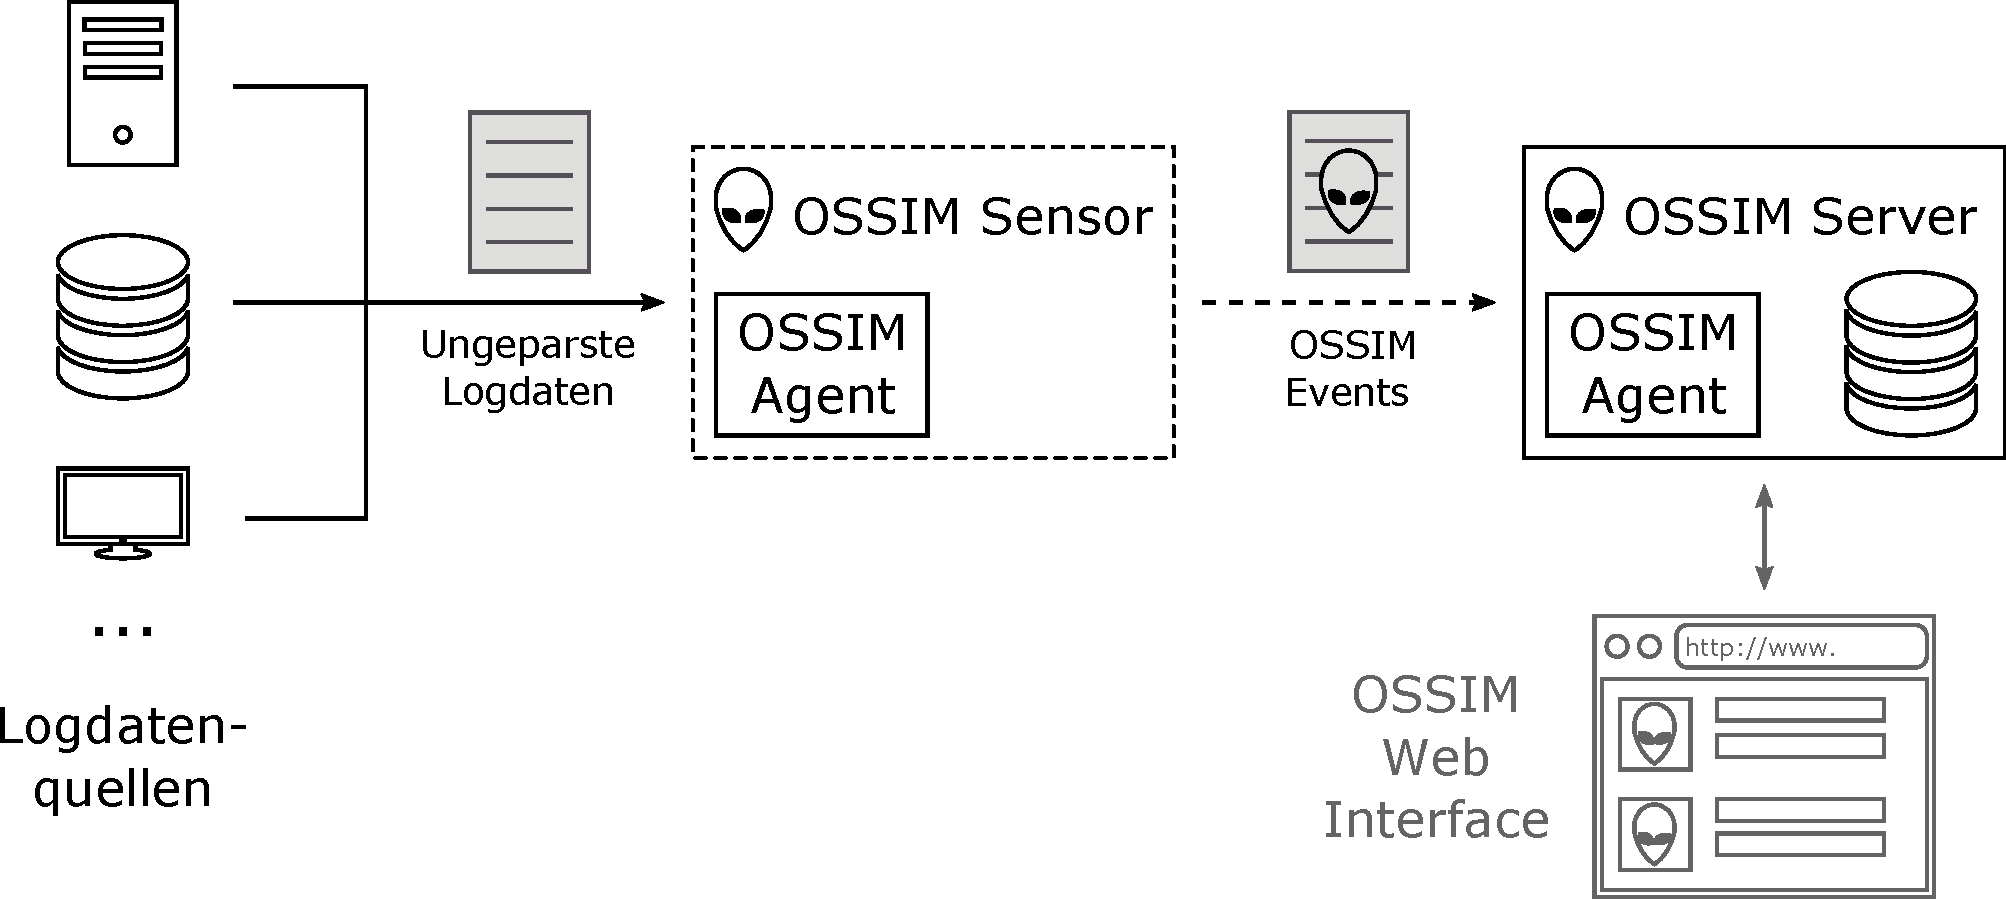
\includegraphics[width=0.9\textwidth]{dia/ossim_log_flow.pdf}
    \caption{High-Level-Übersicht über die OSSIM-Architektur und den Datenfluss.}
    \label{fig:ossim_log_flow}
\end{figure}


\subsection{Parsen von Logdaten in OSSIM}

\label{subsec_state_siem_parsing}

% Quellenarten
% Plugins
% OSSIM-Events
Besonders von Bedeutung für diese Arbeit ist die Verarbeitung von Logdaten. OSSIM ermöglicht es, Logdaten aus unterschiedlichen Quellen entgegenzunehmen bzw. aktiv selber abzurufen und in ein gemeinsames Event-Format zu übersetzen. Hierzu stehen verschiedene Möglichkeiten zur Verfügung:

\begin{itemize}
  \item Entgegennehmen von Daten über das Syslog-Protokoll
  \item Beschaffen von Daten über das SNMP-Protokoll
  \item Entgegennehmen von Daten über proprietäre Protokoll wie SDEE oder WMI
  \item Beschaffen von Daten durch Datenbankabfragen 
\end{itemize}

Unabhängig von der Datenquelle funktioniert die Verarbeitung der Logdaten nach dem immer gleichen Schema. OSSIM bietet die Möglichkeit mitgelieferte oder selber entwickelte Plugins für verschiedene Datenquellen zu aktivieren. Für eintreffende Logdaten überprüft der Agent anhand von regulären Audrücken, ob ein Plugin für das entsprechende Datum zuständig ist. Ist so ein Plugin gefunden, so wird ein neues OSSIM-Event angelegt und anhand der Angaben im Plugin die entsprechenden vorgegebenen Felder des Events gesetzt. Hierbei kann es sich beispielsweise um den Zeitpunkt des Events, IP-Adresse und Port der Datenquelle, einen zu dem Event gehörigen Netzwerkbenutzer oder ereignisabhängige selbstgesetzte Felder handeln. Anschließend folgt die Weiterleitung des Events an den Server.


\section{Pseudonymisierung}

\label{sec_state_pseudonymity}

%pfitzmann2001 - Abschnitt 12
Der Begriff der Pseudonymisierung beschreibt die Benutzung von Pseudonymen zur Identifizierung von Subjekten. Ein Pseudonym (im technischen Sinne) kann nach \cite{pfitzmann2010} als einfache Bitkette betrachtet werden. Es sollte zufällig generiert werden, d.h. vollkommen unabhängig von dem zugehörigen Subjekt oder es betreffenden Eigenschaften sein, um keine Rückschlüsse aus dem Pseudonym selbst zu ermöglichen. Ein Negativbeispiel wäre ein nutzervergebenes Pseudonym, das den Namen des Haustiers enthält. Aber beispielsweise auch eine aufsteigende Nummerierung als Pseudonym könnte durch den hierdurch genauer spezifizierten Erstellungszeitpunkt Rückschlüsse auf das Subjekt hinter dem Pseudonym ermöglichen.

Pseudonymisierung sagt erst einmal lediglich etwas über die Verwendung eines Verfahrens aus, jedoch nichts über die daraus entstehenden Auswirkungen auf die Identifizierbarkeit eines Subjekts oder die Zurechenbarkeit bestimmter Aktionen. Hierfür spielen nach \cite{pfitzmann2001} weitere Eigenschaften von Pseudonymen wie die folgenden eine Rolle:
\begin{itemize}
  \item garantierte Eindeutigkeit von Pseudonymen
  \item Möglichkeit von Pseudonymänderungen
  \item begrenzt häufige Verwendung von Pseudonymen 
  \item zeitlich begrenzte Verwendung von Pseudonymen
  \item Art der Pseudonymserstellung
\end{itemize}

Um die Auswirkungen dieser Eigenschaften einordnen zu können, soll im Folgenden kurz die Pseudonymisierung in zwei Systemen betrachtet und die Relevanz der eben genannten Eigenschaften verdeutlicht werden: Pseudonyme in Mobilfunknetzen und in der Fahrzeug-zu-Fahrzeug-Kommunikation. 

\subsection{Mobilfunknetze}

In Mobilfunknetzen wird zur Identifikation eines Teilnehmers anstelle seiner identifizierenden \textit{International Mobile Subscriber Identity} meist ein Pseudonym -- die \textit{Temporary Mobile Subscriber Identity} (TMSI) -- genutzt, das in bestimmten Situationen gewechselt wird und so Ortung und Bewegungsprofile der Teilnehmer verhindern soll.
In \cite{arapinis2014} beschreiben die Autoren Schwächen der Implementierungen von Mobilfunkstandards in Netzen bei der (Neu-)Vergabe einer TIMSI. Bestimmte Eigenschaften im Bezug auf die Unverkettbarkeit von Pseudonymen und damit auf die Privatsphäre der Nutzer werden in vielen Netzen aufgrund einiger Schwächen nicht erreicht:
\begin{itemize}
  \item Zu seltene Änderung der Pseudonyme
  \item Keine nutzungsabhängige Änderung von Pseudonymen
  \item Pseudonyme werden in verschiedenen Bereichen beibehalten
  \item Anfälligkeit der Neuvergabe für Replay-Angriffe
\end{itemize}
Die letzten beiden Schwächen sind für den Anwendungskontext dieser Arbeit nicht relevant, aber die zeit- und aktivitätsabhängige Neuvergabe von Pseudonymen müssen auch hier beachtet und umgesetzt werden.

\subsection{VANets}

Ein anderer Bereich, der sich besonders mit der Nutzung von Pseudonymen beschäftigt hat, ist die Forschung an Vehicular Ad Hoc Networks (VANets). Hierbei handelt es sich um Netzwerke für die Kommunikation zwischen Fahrzeugen, die beispielweise für die Datenübermittlung zur Bremserkennung naher Fahrzeuge oder die Stauerkennung genutzt werden können. Um die Privatsphäre der Fahrzeughalter zu schützen, wird für die Kommunikation in vielen Ansätzen auf die Verwendung von Pseudonymen gesetzt. So soll sich beispielsweise das Anlegen von Bewegungsprofilen verhindern lassen.\\
Unter anderem in \cite{dotzer2005} und \cite{petit2015} widmen sich die Autoren der Nutzung von Pseudonymen in VANets und den besonderen Anforderungen, die diese erfüllen müssen -- insbesondere auch im Hinblick auf die Häufigkeit von Pseudonymwechseln. Es ergibt sich, dass die Häufigkeit und Situation\footnote{
  Es werden beispielweise Lösungen vorgestellt, die abhängig von Geschwindigkeitsänderungen, einer gewissen Anzahl anderer Fahrzeuge oder besonderen Verkehrssituationen wie Kreuzungen die Pseudonymänderung vornehmen. Das Ziel ist hier immer die Möglichkeit der Pseudonymverkettung bzw. der Bewegungsprofilerstellung durch die äußere Situation der Pseudonymänderung zu erschweren.
}, in der Pseudonymwechsel stattfinden sollten, abhängig vom gewünschten Grad an Anonymität bzw. Angreifermodell sind und außerdem gegenüber Sicherheitsanwendungen\footnote{
  Beispielsweise wäre zur VANet-basierten Kollisionsvermeidung eine Verkettung von Orten, an denen sich ein Fahrzeug zu verschiedenen Zeitpunkten befindet, erstrebenswert.
}  abgewogen werden müssen.\\
Bei der Nutzung von Pseudonymen in VANets handelt es sich natürlich um eine Anwendung mit anders gelagerten Prioritäten im Vergleich zu dem Kontext dieser Arbeit. Dennoch wird deutlich, dass die Strategie zum Pseudonymwechsel stark von der Anwendungssituation abhängig ist. Bezogen auf den hier vorliegenden Anwendungsfall werden insbesondere Besonderheiten der Datenquelle, wie die Häufigkeit von auftretenden Überwachungsdaten, und Anforderungen an die Verknüpfbarkeit von Ereignissen der auf den Daten beruhenden Anomalieerkennung zu beachten sein.

% Perfect Forward Privacy

In \cite{schaub2009} stellt der Autor eine weitere Anforderung an die Nutzung von Pseudonymen in VANets, die jedoch nicht nur für diesen speziellen Anwendungsfall relevant ist: Er verlangt, dass die Aufdeckung eines Pseudonyms keine Informationen über die Identität eines Nutzers im Bezug auf andere Pseudonyme ermöglichen sollte. Diese Eigenschaft bezeichnet er als \textit{Perfect Forward Privacy}\footnote{
  Die Bezeichnung ist an \textit{Perfect Forward Secrecy} angelehnt. Diese Eigenschaft beschreibt ein ähnliches Verhalten bei der verschlüsselten Kommunikation: Ein Angreifer, der in den Besitz des Langzeitschlüssels eines Kommunikationspartners kommt, sollte trotzdem nicht in der Lage sein, bereits aufgezeichnete Nachrichten entschlüsseln zu können.
}.

\subsection{Pseudonymisierung im zu entwickelnden System}

% - Pseudonymgenerierung
% - Pseudonymwechsel zeit und datenmengenabhängig
%   leider nicht genauer, da sowohl datenquellen als auch anomaliedings nicht klar
%   daher parameter ermöglichen
% - PFP in DB umsetzen

Aus diesen Vorüberlegungen können nun die Rahmenbedingungen der in dieser Arbeit verwendeten Pseudonymisierung aufgestellt werden.
Pseudonyme sollten als zufällig gewählte Bitketten hinreichender Länge gewählt werden. Ihre Eindeutigkeit muss sichergestellt werden.

Wie auch in den Beispielen deutlich wurde, müssen Pseudonyme abhängig von dem Anwendungsszenario in bestimmten Fällen für einen Benutzer gewechselt werden. In dem hier vorliegenden Anwendungsfall, in dem Pseudonyme für die Zuordnung von eintreffenden Überwachungsdaten in Unternehmensnetzen genutzt werden, sind insbesondere die Zeitabhängigkeit sowie die Abhängigkeit von der Nutzungshäufigkeit für die Pseudonymwechselstrategie ausschlaggebend. Verschiedene Nutzeraktionen sollten nur in einem gewissen zeitlichen Rahmen und nur in einer gewissen Häufigkeit verkettbar sein. Es handelt sich also um eine schwächere Form der Transaktionspseudonyme, bei der ein Pseudonym je nach Pseudonymwechselstrategie nur für eine bestimmte Anzahl an Ereignissen verwendet wird.

Eine über diese generelle Aussage hinausgehende Bewertung davon, wie diese Abhängigkeiten konkret zu implementieren sind, ist jedoch im Rahmen dieser Arbeit nicht zu leisten. Hierfür sind zwei Gründe ausschlaggebend:
\begin{itemize}
  \item Sie hängen stark von den Eigenschaften der Datenquellen ab, die die Überwachungsdaten liefern. Beispielsweise wäre das Datenprofil, das von einem elektrischen Türschließsystem geliefert wird, sehr unterschiedlich zu dem, das Zugriffe auf einen Netzwerkspeicher protokolliert. Im ersten Fall würden im Allgemeinen selten Daten anfallen, die zudem durch die Anwendung von Hintergrundwissen (Benutzer wird beim Betreten eines Raumes beobachtet) eher zur Aufdeckung eines Pseudonyms führen könnten. Hier wären wahrscheinlich häufige nutzungsabhängige Wechsel angebracht. Eventuell wäre sogar der Extremfall einer einmaligen Pseudonymvergabe pro Aktion in Erwägung zu ziehen.\\
  Im zweiten Fall hingegen würden im Allgemeinen häufig Daten anfallen und erst die Verkettung dieser Daten könnte hilfreiche Rückschlüsse auf vorliegende Anomalien liefern. Ein einzelner Datenzugriff hätte meist wenig Aussagekraft, wohingegen ein massenhafter Zugriff beispielsweise auf die Kundendatenbank eines Unternehmens durch einen gekündigten Mitarbeiter möglicherweise auf Datendiebstahl schließen lassen könnte.
  
  \item Weiterhin muss die Pseudonymwechselstrategie auch abhängig von der später auf den pseudonymisierten Überwachungsdaten auszuführenden automatisierten Anomalieerkennung sein. Je nachdem welche Verfahren auf Daten aus welchen Datenquellen eingesetzt werden sollen, könnte auch hier unterschiedliche Verknüpfbarkeit der Daten erforderlich sein. Hieraus ergibt sich auch ein Spannungsfeld zwischen den Anforderungen der Anomalieerkennung gegenüber der Verknüpfbarkeit der Daten und damit der Privatsphäre der Arbeitnehmer.
\end{itemize}

Aus diesen Gründen wird eine parameterabhängige Pseudonymwechselstrategie implementiert, die sowohl zeit- als auch die nutzungsabhängige Wechsel ermöglicht. Wie lange bzw. häufig ein Pseudonym verwendet wird, kann so in konkreten Anwendungen mit gesetzten Rahmenbedingungen beurteilt und gesetzt werden.
% Digitalgipfel
Dieses Vorgehen wird auch in den \textit{Leitlinien für die rechtssichere Nutzung von Pseudonymisierungslösungen unter Berücksichtigung der Datenschutz-Grundverordnung} beschrieben: \glqq Abhängig vom Anwendungsfall sind – zeit- oder datenvolumenabhängig – geeignete Intervalle zu definieren, in denen ein Wechsel [...] erfolgt.\grqq{}\cite{schwartmann2017}

Weiterhin wird angestrebt für die Pseudonyme bzw. ihre Aufdeckung die erwähnte Perfect Forward Privacy zu ermöglichen. Die konkrete Umsetzung dieser Eigenschaft wird in einem späteren Abschnitt beschrieben werden.

\section{Schwellwertschemata}

\label{sec_state_threshold}

%\subsection{Schemata}

% - RSA signing/decryption \cite{frankel1997proactive} proactive
% - RSA signing/decryption \cite{gennaro1996robust} robust efficient
% - RSA signign/decryption \cite{rabin1998simplified} robust proactive
% - RSA signing \cite{nguyen2005}
% - RSA signing \cite{shoup2000practical}
% - Paillier encryption \cite{damgard2001, fouque2000sharing} -> homomorphic for electronic voting
% - DSS signing \cite{gennaro1996robustdss}
% - Schnorr \cite{stinson2001provably}



Aufbauend auf den Ideen von Shamir und Blakley und den ersten Ideen zu kryptographischen Schwellwertschemata wurden für verschiedene Algorithmen und Anwendungsfälle Schemata mit unterschiedlichen Eigenschaften entwickelt.

\subsection{Übersicht}

Eine Vielzahl von Veröffentlichungen behandlen das Problem der verteilten Erstellung von Signaturen: Die in \cite{shoup2000practical} entwickelte Lösung basiert auf dem RSA-Verfahren, \cite{gennaro1996robustdss} erweitert den DSS-Standard um ein Schwellwertschema und \cite{stinson2001provably} entwickelt ein Schema zur verteilten Signatur mittels Schnorr-Signaturen.\\
Weitere Forschungen haben sich mit der Entwicklung von RSA-basierten Schwellwertschemata zur verteilten Entschlüsselung beschäftigt, die im Kontext dieser Arbeit genutzt werden \cite{frankel1997proactive, gennaro1996robust, rabin1998simplified}. \\
Ein zusätzliches Verfahren, das im Zusammenhang mit verteilter Entschlüsselung Aufmerksamkeit erfuhr, ist das Paillier-Kryptosystem. In \cite{damgard2001} und \cite{fouque2000sharing} entwickelten die Autoren auf diesem System basierte Schwellwertschemata, die insbesondere durch ihre homomorphe Eigenschaft hervorstechen und dadurch im Bereich der elektronischen Wahlsysteme genutzt werden können.\\
Einen Überblick über weitere Veröffentlichungen in diesem Bereich bieten beispielsweise \cite{desmedt1997some}, \cite{gemmell1997} und \cite{desmedt1993}.

\subsection{ElGamal-basiertes Schwellwertschema}

\label{sec_state_threshold_scheme}

Ein Verfahren zur \textit{Threshold Decryption}, das auf auf einer geschickten Kombination von Shamir's Secret Sharing (Abschnitt \ref{sec_basics_threshold_shamir}) und des ElGamal-Kryptosystems (Abschnitt \ref{sec_basics_threshold_elgamal}) basiert, veröffentlichten die Autoren in \cite{DesmedtFrankel1990}. Aufbereitete Darstellungen lassen sich in \cite{katz2014} und \cite{boneh2016} finden. \\
Es ist eines der ersten veröffentlichten Schwellwertschemas und erfuhr dadurch viel Beachtung und entsprechend viele aufbauende Arbeiten, die Verbesserungen vorschlugen. Durch die hinterliegende Mathematik bietet das Schema einfachere Umsetzbarkeit (auch von Erweiterungen wie dezentraler Schlüsselgenerierung) gegenüber RSA\footnote{
  Das ElGamal-Verfahren nutzt zur Berechnung eine öffentlich bekannter Ordnung (sie ist Teil des öffenltichen Schlüssels). Im Gegensatz dazu werden Berechnungen bei RSA in \(\Phi(n)\) ausgeführt, das jedoch nicht öffentlich vorliegen darf \cite{nguyen2005}.
}. Dies gilt ebenso gegenüber den Paillier-basierten Schemata -- deren homomorphe Eigenschaften in dieser Arbeit nicht benötigt werden. Aus diesen Gründen fiel die Wahl des in dieser Arbeit umzusetzenden Schemas auf das genannte Verfahren.\\
Der Rest dieses Abschnitts stellt das Verfahren nun entsprechend den in Abschnitt \ref{sec_basics_threshold_thresholddecryption} aufgeführten Algorithmen eines Threshold-Public-Key-Decryption-Systems im Detail vor.

%\subsection{Umzusetzendes kryptographisches Schwellwertschema}

%- Desmedt und Frankel, aufbereitet auch in Katz und Boneh.

%- Verfahren basierend auf Shamir und ElGamal

%- Analog zu basics-threshold-formal (zentrale) lässt sich das Verfahren in 4 Phasen unterteilen

\textbf{Algorithmus G: Schlüsselgenerierung}

In dem Verfahren wird für die Schlüsselgenerierung eine zentrale, vertrauenswürdige Instanz vorausgesetzt, die den öffentlichen Schlüssel und die später benötigten Shares des geheimen Schlüssels erzeugt und verteilt. 

Zur Erzeugung werden zwei Primzahlen \(p\) und \(q\) mit der Eigenschaft \(p = 2q + 1\) - bekannt als sichere Primzahl bzw. Sophie-Germain-Primzahl - benötigt. Weiterhin ist ein Generator der Untergruppe der Ordnung \(q\) von \(\mathbb{Z}_p^*\) notwendig.

Der (temporär erstellte) geheime Schlüssel \(a \in \mathbb{Z}_q\) wird analog zu der Schlüsselgenerierung im ElGamal-Verfahren zufällig gewählt. Aus ihm wird der öffentliche Schlüssel \(pk = g^a \mod p\) berechnet.\\
Der geheime Schlüssel wird anschließend analog zu Shamirs Secret Sharing in \(\mathbb{Z}_q\) in einzelne Shares \((x_i, y_i) = (x_i, q(x_i))\) aufgeteilt und diese an die Teilnehmer verteilt. Anschließend werden diese Werte gelöscht, so dass nur noch die Teilnehmer im Besitz ihrer Shares und damit in der Lage sind, Schlüsseltexte zu entschlüsseln.

\textbf{Algorithmus E: Verschlüsselung}

Anschließend kann ein Klartext mithilfe von \(pk\) analog zu dem ElGamal-Verfahren 
%(siehe Abschnitt \ref{sec_basics_threshold_elgamal}) 
verschlüsselt werden. So erhält man \((v,c) = (g^k, m \cdot g^{ak})\) für ein durch den Sender zufällig gewähltes \(k \in \mathbb{Z}_q\).

\textbf{Algorithmus D: Partielle Entschlüsselung}

Jeder Besitzer eines Shares \((x_i, y_i)\) kann nun für den zu entschlüsselnden Schlüsseltext \((v,c)\) seine partielle Entschlüsselung \((x_i, v^{y_i})\) berechnen und diese an eine zentrale Instanz, den Combiner, senden. Empfängt dieser mindestens \(t\) partielle Entschlüsselungen\footnote{
  Zur Erinnerung: \(t\) beschreibt die Mindestzahl zur Entschlüsselung benötigter Shares des Schwellwertschemas.
}, so kann er den Klartext wiederherstellen.

\textbf{Algorithmus C: Kombination}

Hierzu berechnet der Combiner die Lagrange-Koeffizienten \(\lambda_i \in \mathbb{Z}_q\) wie in Shamir's Secret Sharing beschrieben\footnote{
  In diesem Abschnitt gilt \(i \in C\). \(C\) stellt dabei die Menge der Indizes der beteiligten Sharebesitzer dar. Es gilt also \(C \subseteq \{1, \dots, n\}\) und \(| C | \ge t\).
}. Anschließend kann
 
\[g^{ak} = \prod_{i=1}^k (v^{y_i})^{\lambda_i}\]

berechnet werden. Dies funktioniert, da 

\[
\prod_{i=1}^k (v^{y_i})^{\lambda_i} = 
\prod_{i=1}^k (g^k)^{y_i \cdot \lambda_i} = 
(g^k)^{\sum_{i=1}^{k} y_i \cdot \lambda_i} \overset{(*)}{=}
(g^k)^a
\]

gilt. Der letzte Schritt \((*)\) folgt direkt aus dem zugrundeliegenden Secret-Sharing-Schema und ist in dieser Form bereits in Abschnitt \ref{sec_basics_threshold_shamir} zu finden.

Anschließend kann der Klartext als \(m = c \cdot (g^{ak})^{(-1)}\) wiederhergestellt werden. 

\subsection{Verteilte Schlüsselgenerierung}

\label{sec_state_threshold_distributed}

Ein Nachteil dieses Verfahrens in der Phase der Schlüsselgenerierung ist, dass für die Generierung des geheimen Schlüssels und der daraus resultierenden Shares eine zentrale und vertrauenswürdige Instanz notwendig ist. Diese Problematik wurde bereits in Abschnitt \ref{subsec_impl_requirements_threshold} dargestellt und Auswirkungen in Abschnitt \ref{subsec_impl_requirements_attackermodel} betrachtet.

In \cite{pedersen1991} wurde vom Autor eine Möglichkeit der verteilten Schlüsselgenerierung für das dargestellte Verfahren vorgeschlagen, die von den Autoren in \cite{gennaro1999} noch verbessert wurde. 

Das Verfahren besteht aus zwei Phasen: In der ersten Phase wird von allen potentiellen Share-Besitzern ein \textit{Verifiable Secret Sharing Scheme}\footnote{
  Verifiable Secret Sharing Schemes sind Secret Sharing Schemes, die es den Share-Besitzern erlauben zu überprüfen, ob ihre Shares konsistent sind, d.h. ob es möglich ist aus den Shares ein gemeinsames Geheimnis wiederherzustellen. Bei dem in Abschnitt \ref{sec_basics_threshold_shamir} vorgestellten Secret Sharing nach Shamir ist dies beispielsweise nicht der Fall. Ein bösartiger Erzeuger von Shares könnte für jeden Beteiligten ein anderes Geheimnis benutzen, so dass bei der Rekonstruktion abhängig von beteiligten Share-Besitzern unterschiedliche Geheimnisse erhalten werden.
} (VSS) nach Pedersen ausgeführt, das dafür sorgt, dass anschließend alle ehrlichen Beteiligten jeweils im Besitz eines Shares sind, die zusammengenommen den geheimen Schlüssel \(x\) bilden (der jedoch nirgendwo vorliegt oder im Laufe des Verfahrens vorlag). In der zweiten Phase wird ein VSS nach Feldman dazu genutzt, den gemeinsamen öffentlichen Schlüssel \(y = g^x\) auf eine Weise zu berechnen, die wiederum dafür sorgt, dass der geheime Schlüssel nirgendwo vorliegen muss. Auf diese Weise wird die vertrauenswürdige Instanz vermieden und es ist trotzdem sichergestellt, dass die ehrlichen Beteiligten im Besitz von Shares sind, die die Verwendung des kryptographischen Schwellwertschemas so ermöglichen wie im letzten Abschnitt für das Verfahren mit zentraler Schlüsselgenerierung vorgestellt.

\subsection{ECC-ElGamal}

\label{sec_state_threshold_ecc}

Eine andere Verbesserung für das Verfahren ist die Verwendung von \textit{Elliptic Curve Cryptography}. Hier werden die Berechnungen des ElGamal-Verfahrens nicht mehr in der beschriebenen Untergruppe von \(\mathbb{Z}_p^*\), sondern als Operationen auf elliptischen Kurven über endlichen Körpern ausgeführt \cite{koblitz1987elliptic}.

Vorteil der Verwendung ist eine deutlich geringere benötigte Schlüssellänge für vergleichbare Sicherheit im Vergleich zu dem ursprünglichen Verfahren\footnote{
  Das BSI gibt eine Schlüssellänge von etwa 250 Bits für ECC-Verfahren als vergleichbare Sicherheit erreichend zu 2000-Bit-Schlüsseln für Verfahren wie RSA oder auf dem Diskreten-Logarithmus-Problem beruhenden Verfahren an \cite{bsi2018}.
}. Durch diese kürzeren Schlüssel werden auch Berechnungszeit und Speicherverbrauch trotz komplexerer Berechnungen eingespart werden.

\subsection{Verallgemeinerte Schwellwerte}

\cite{ito1989secret} \textit{Access structure}
\todo{Schreiben!}

\subsection{Existierende Implementierungen}

\label{sec_state_threshold_existing_impl}

Auch nach umfangreicher Recherche ließ sich keine quelloffene, kryptographisch überprüfte und lizenzrechtlich nutzbare Bibliothek finden, die das gewünschte Schwellwertschema implementiert. Es gab verschiedene verwandte Lösungen wie Civitas\footnote{
  Civitas -- A secure voting system. http://www.cs.cornell.edu/projects/civitas/
} oder Helios\footnote{
  Helios Voting. https://heliosvoting.org/
}, die jedoch alle eng mit dem Anwendungskontext der elektronischen Wahl verknüpft waren und dadurch andere Anforderungen erfüllten als sie für diese Arbeit erforderlich sind. Aus diesem Grund wird das beschriebene Schwellwertschema gezwungenermaßen in Teilen selbstständig implementiert.

\section{Searchable Encryption}

\todo{To be written...}